\mychapter{Visão geral dos exames}\label{ch:exames}

A realização dos exames desempenha um papel fundamental no MCTest, sendo o elemento central do sistema. Nessa etapa, é possível ter a flexibilidade de incluir uma ou várias turmas de estudantes em um exame, selecionar as questões que farão parte dele, decidir sobre o formato de impressão (como uma questão por folha ou de maneira ecologicamente sustentável, com várias questões por folha), determinar a quantidade de variações a serem criadas e escolher se o exame será impresso ou enviado por e-mail aos estudantes, entre outros aspectos relevantes.

Neste capítulo, será fornecida uma visão geral da tela de exames utilizada no MCTest. Como essa tela é extensa, ela será explicada em partes.

Adicionalmente, nos capítulos subsequentes, serão abordadas as diferentes modalidades de exames já utilizadas, contendo:
(1) Questões com apenas o quadro de respostas (QR);
(2) Questões com QR+QT, incluindo os enunciados;
(3) QTs exclusivamente, que requerem correção manual sendo enviadas aos estudantes por e-mail;
(4) QTs exclusivamente, nas quais os estudantes devem fornecer soluções, como exercícios de programação (EPs) em atividades VPL do Moodle.
Além disso, será tratada a combinação desses estilos distintos em um único exame.

\section{Acesso à tela de exames}\label{sec:telaExame}

Após efetuar o \textit{login}, o professor cadastrado em uma disciplina terá acesso à tela de exames no menu superior direito. Ao acessar essa tela, ilustrada na Figura \ref{fig:cap06_figExame}, o professor poderá observar que ainda não foram criados exames. Para iniciar o processo de criação de um novo exame, basta clicar no botão ``Criar um novo Exame'' disponível nessa mesma tela.

\begin{figure}[htbp]
  \centering
  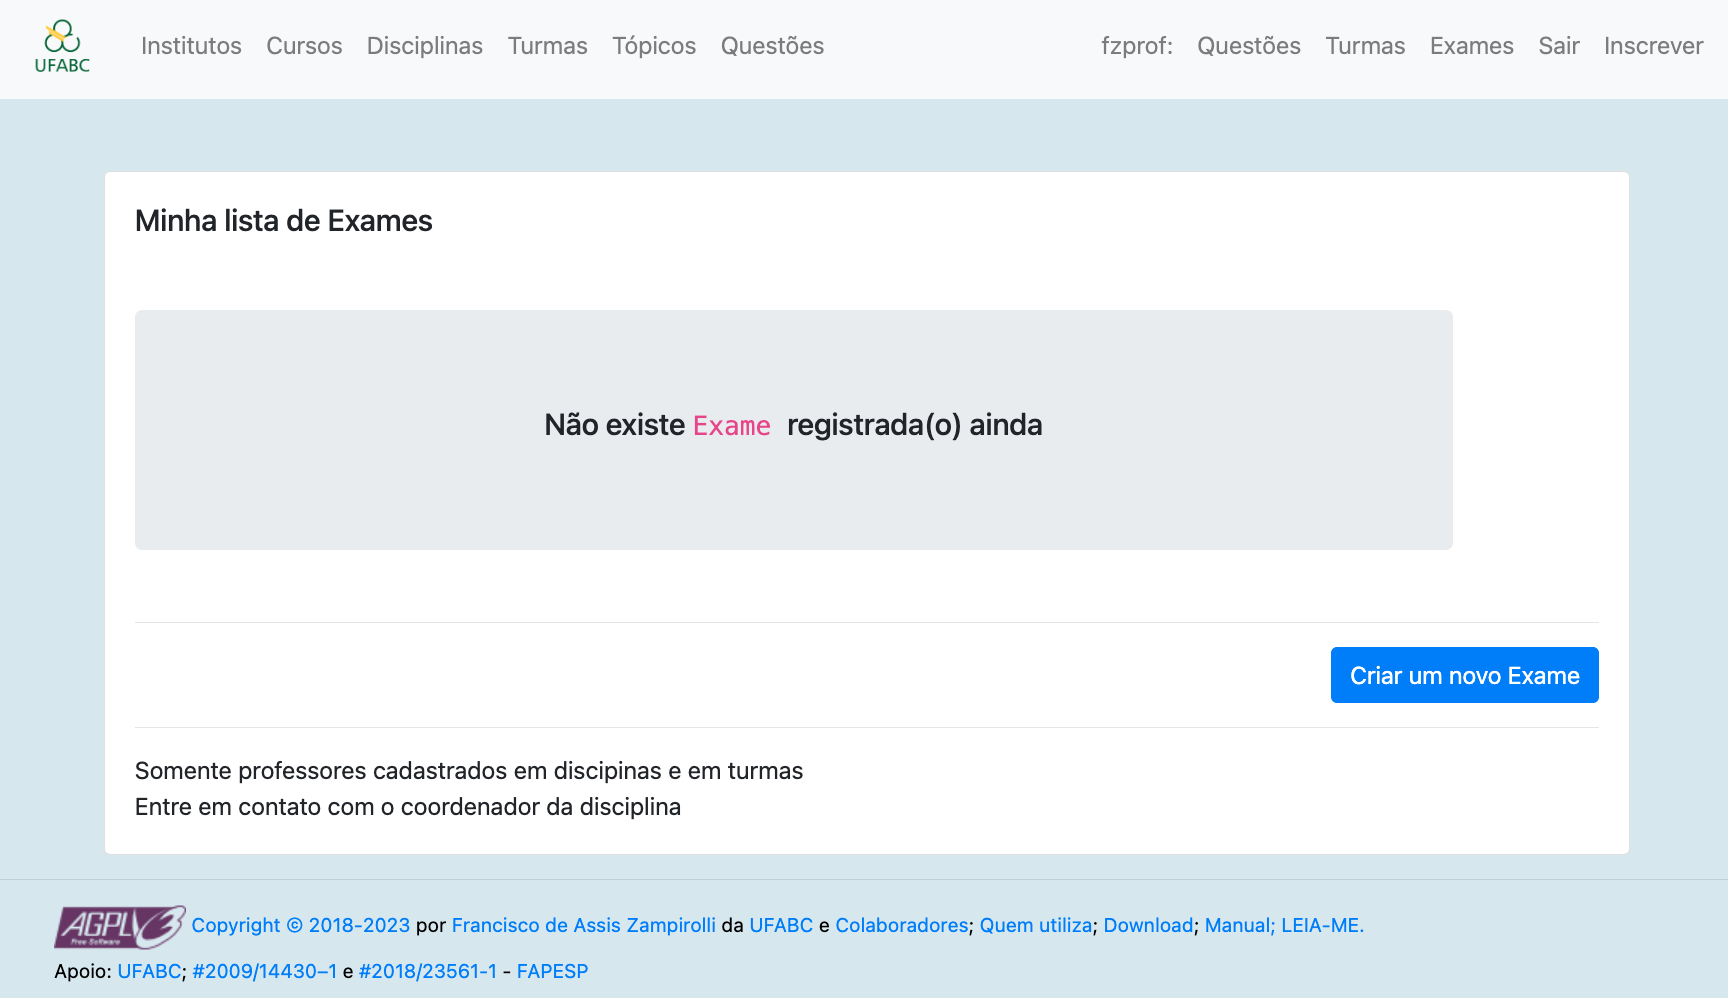
\includegraphics[width=0.9\textwidth]{cap06_figExame.png}
  \caption{Tela de exames do professor.}
  \label{fig:cap06_figExame}
\end{figure}

Na tela de criação de um novo exame (consulte a Figura \ref{fig:cap06_figExameCria}), é necessário selecionar uma turma com pelo menos um estudante e atribuir um nome ao exame. Em seguida, clique no botão ``Salvar''. A criação de turma por um professor foi apresentada nas Seções \ref{sec:turma} -- \nameref{sec:turma} e \ref{sec:professorCriarTurma} -- \nameref{sec:professorCriarTurma}.

\begin{figure}[!t]
  \centering
  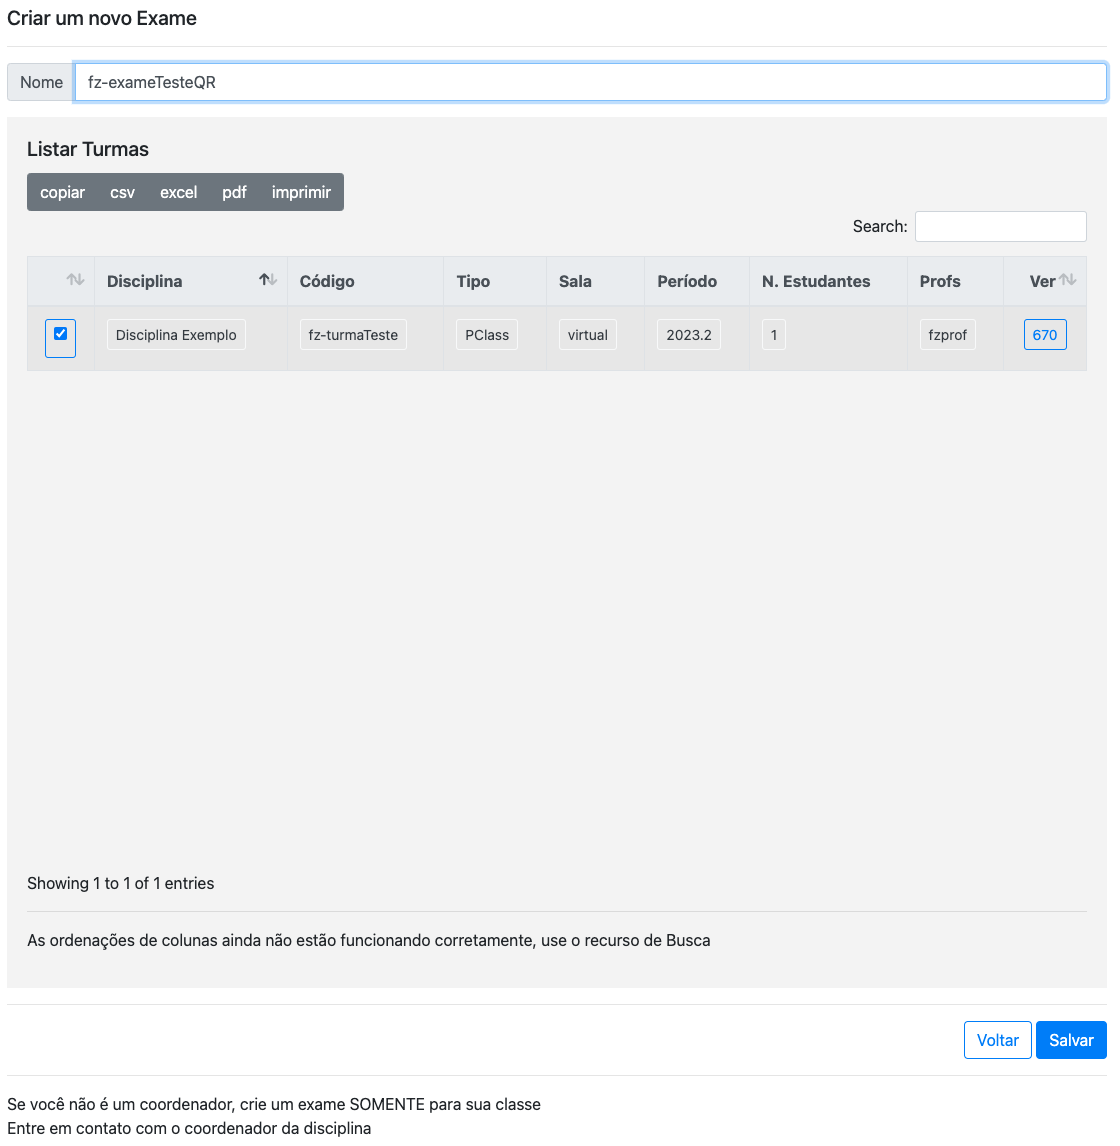
\includegraphics[width=0.9\textwidth]{cap06_figExameCria.png}
  \caption{Tela para criar um novo exame.}\vspace{-3mm}
  \label{fig:cap06_figExameCria}
\end{figure}

\begin{mybox}{corCopia}{\textbf{Atenção:\\\vspace{-3mm}\hrule\vspace{1mm}}}
\begin{enumerate}
    \item  É essencial ressaltar que um exame só pode ser criado se estiver associado a uma turma criada pelo professor. Portanto, antes de excluir uma turma, certifique-se de apagar todos os exames associados a ela;
    \item  Ao acessar a tela de atualização do exame, é extremamente importante preencher os campos com muita atenção. Essa parte do sistema é especialmente sensível e requer a criação de várias mensagens de erro para lidar com o preenchimento incorreto dos campos.
\end{enumerate} 
\end{mybox}

Após a criação do exame, é possível realizar atualizações e configurar todos os atributos necessários para sua conclusão. Devido à extensão dessa parte na versão atual do MCTest, a tela de atualização de exame foi dividida em várias seções, que serão apresentadas a seguir. A tela de exame pode ser acessada por meio do botão ``Atualizar'' exibido na Figura \ref{fig:cap06_figExame} correspondente ao exame em questão recém criado.

Além disso, antes de prosseguir com a explicação detalhada das seções, é possível gerar um PDF do exame com as configurações padrão ao clicar no botão ``Cria-PDF'', conforme detalhado na próxima seção. Esse PDF é ilustrado na Figura \ref{fig:cap06_figExamePDF_QRpadrao}.

\begin{figure}[htbp]
  \centering
  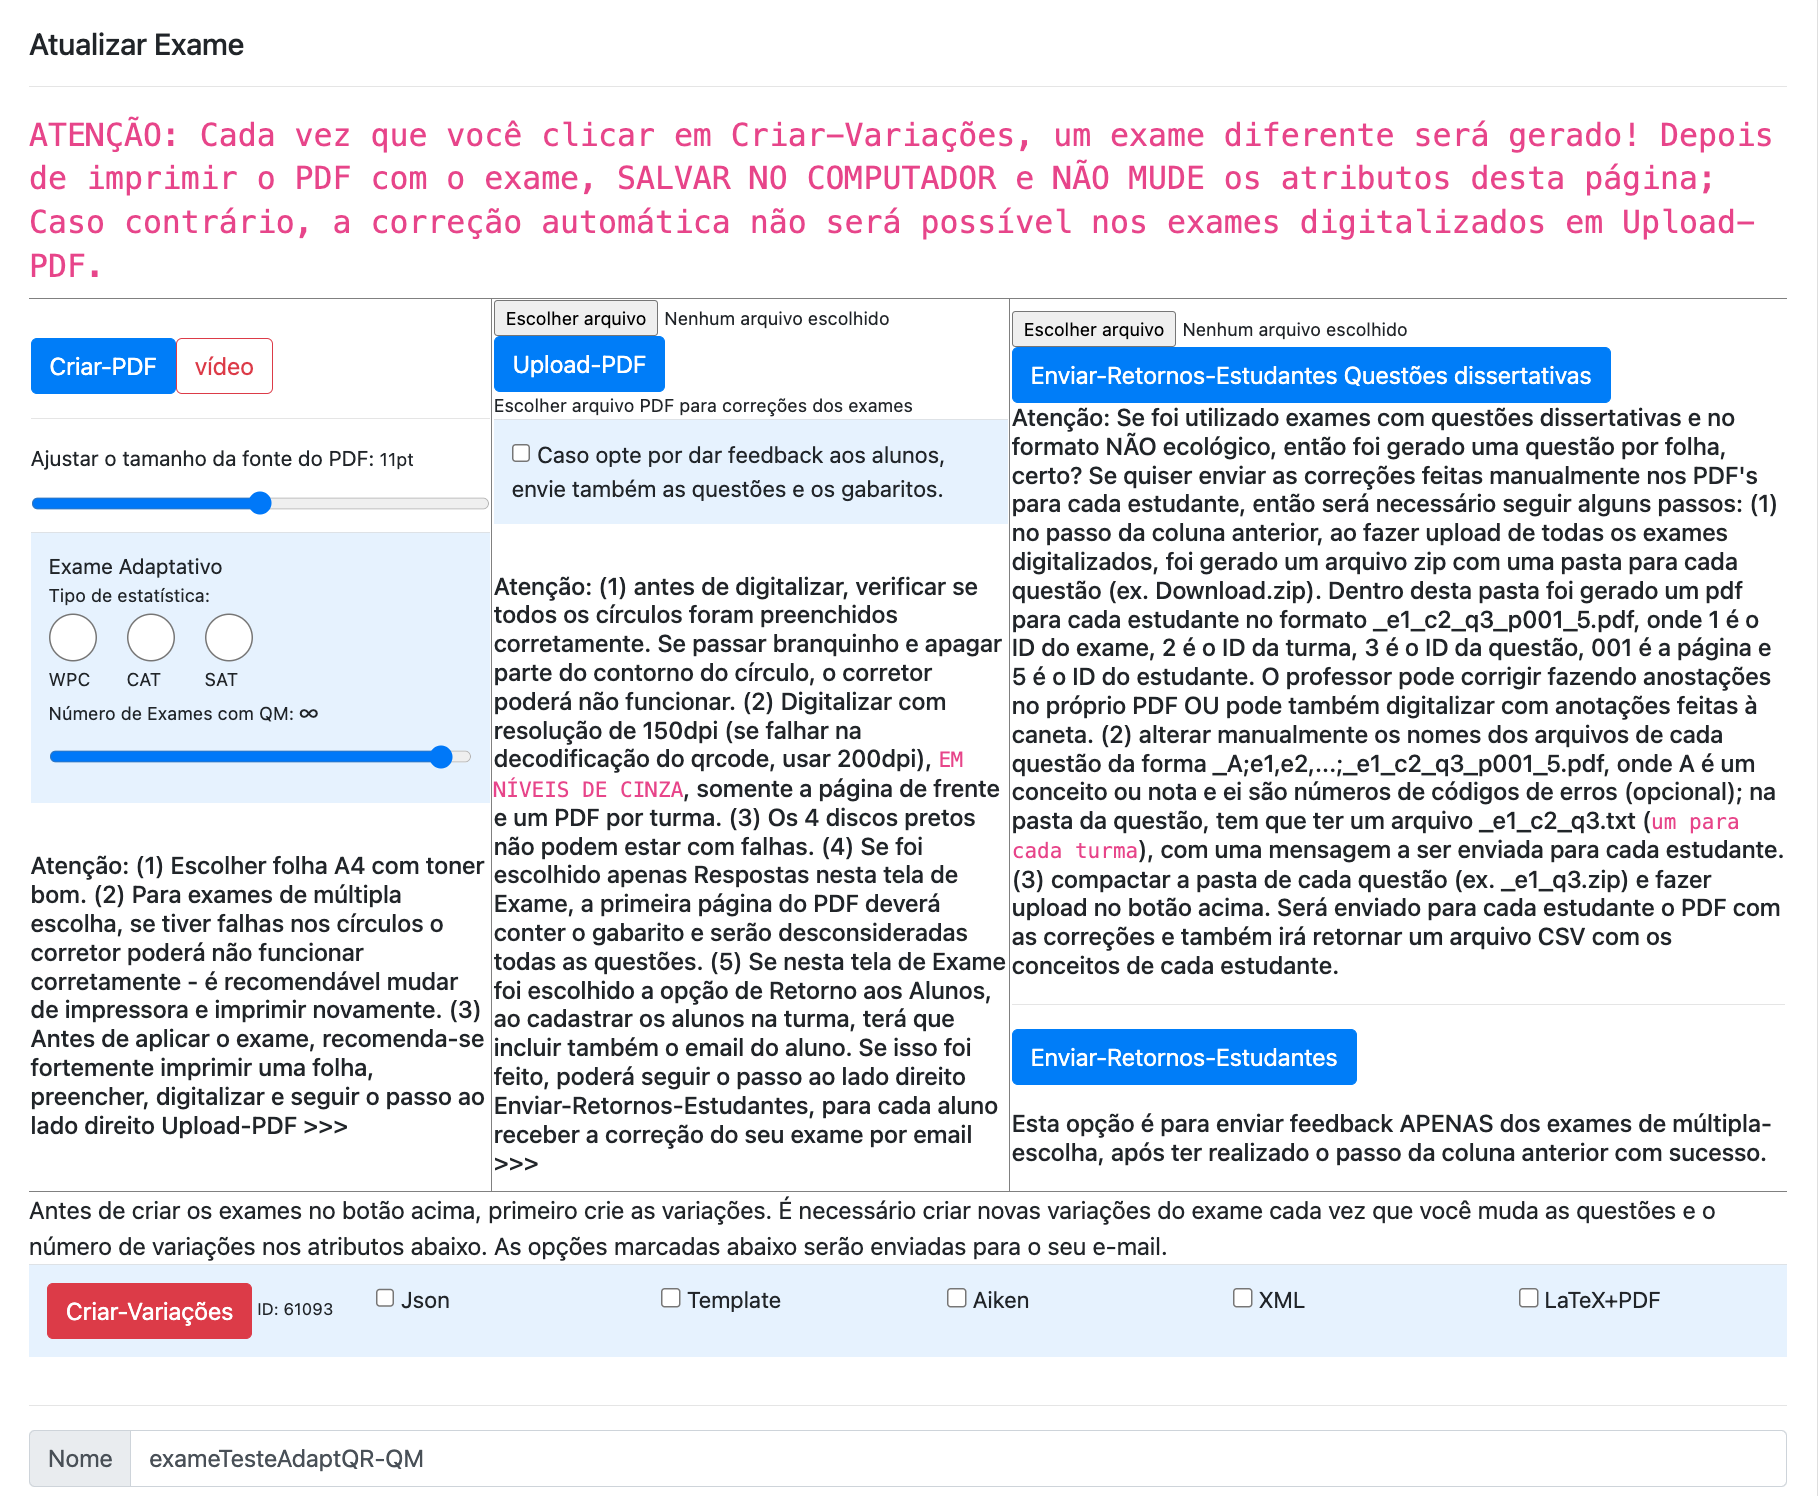
\includegraphics[width=0.9\textwidth]{cap06_figExamePDF_QRpadrao.png}
  \caption{Recorte do PDF gerado com as configurações padrão, contendo apenas o cabeçalho e o QR.}
  \label{fig:cap06_figExamePDF_QRpadrao}\vspace{-3mm}
\end{figure}

\section{Recorte I da tela de exame}\label{sec:exameRecorte1}

Na Figura \ref{fig:cap06_figExameAtualiza1}, é apresentado o Recorte I da tela de atualização de exame, que contém os principais botões para a criação e correção de exames. Cada um desses botões ou combinações foi submetido a experimentos e será detalhado em capítulos futuros deste livro. Esses capítulos fornecerão informações mais específicas sobre a utilização e os resultados dessas funcionalidades.

\begin{figure}[!t]
  \centering
  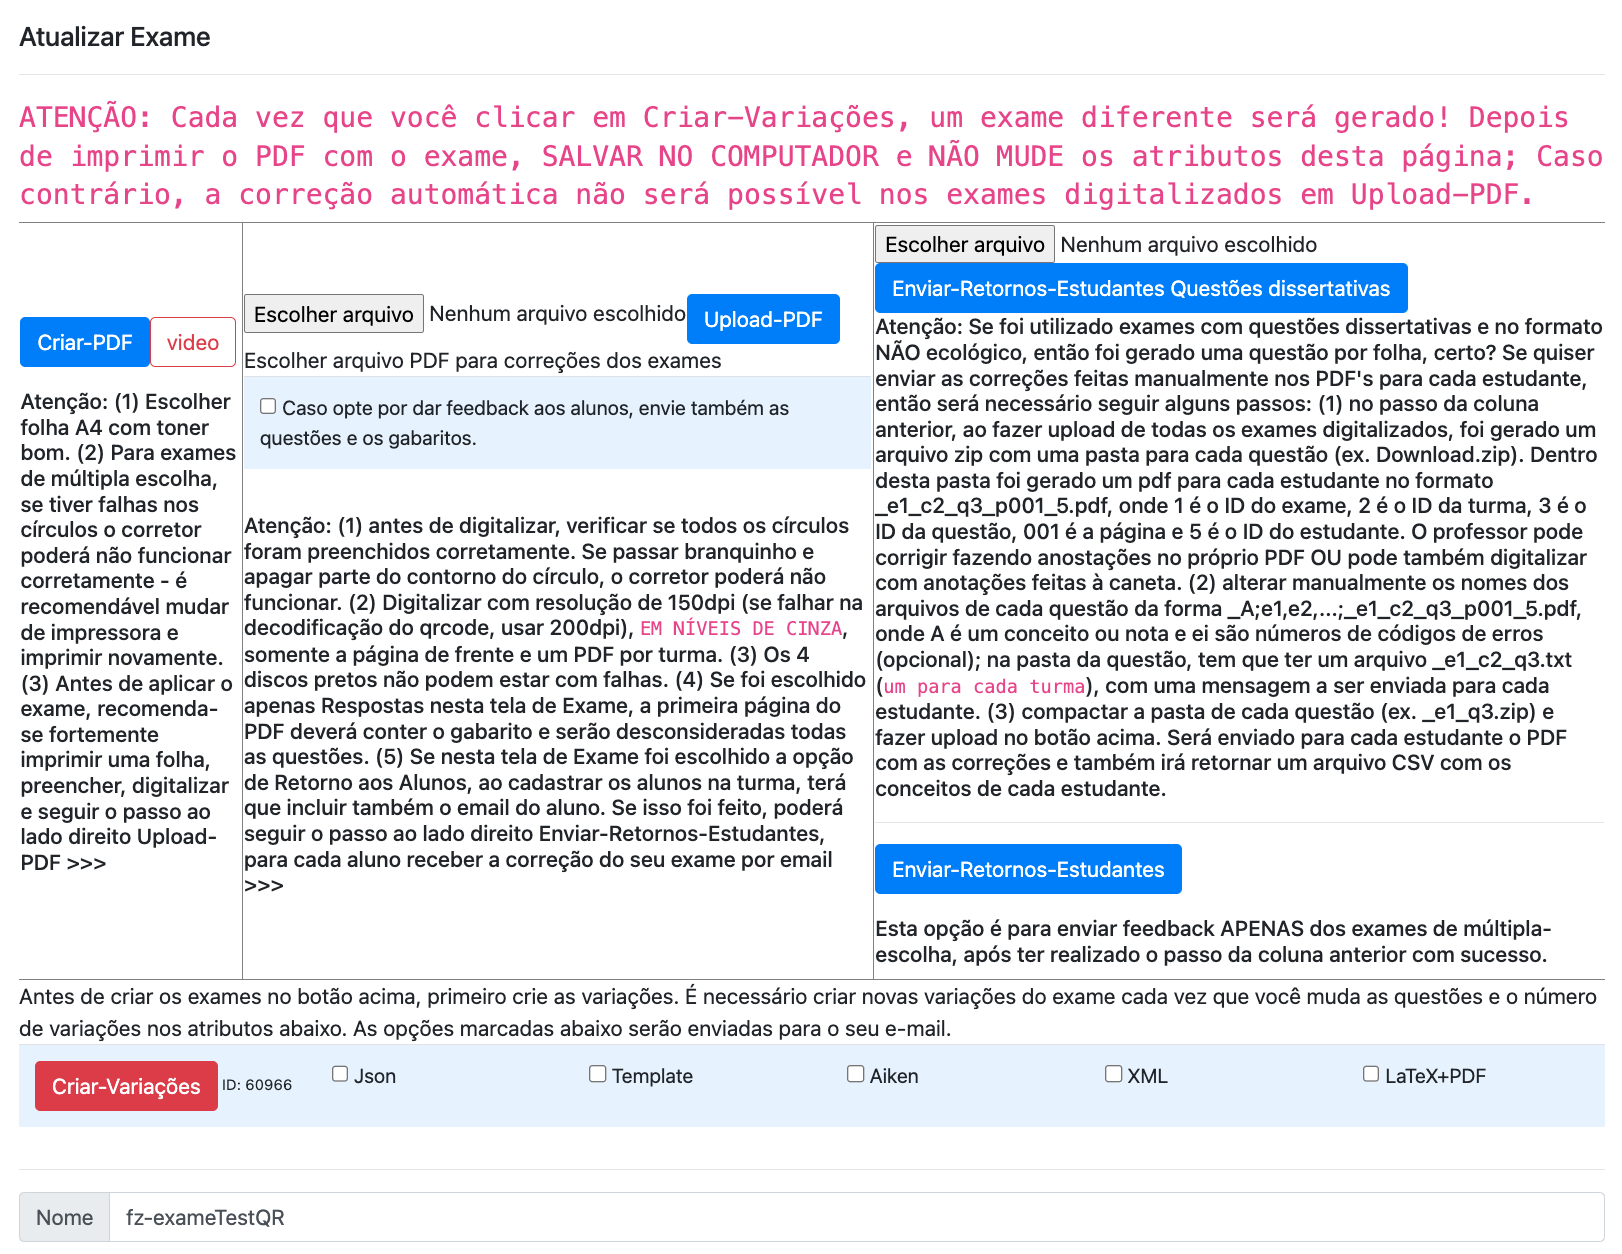
\includegraphics[width=0.9\textwidth]{cap06_figExameAtualiza1.png}
  \caption{Recorte I da tela de exame -- ver explicações no texto sobre os botões.}
  \label{fig:cap06_figExameAtualiza1}\vspace{-3mm}
\end{figure}

\subsection{Área à esquerda}\label{sec:areaEsquerda}

É importante ressaltar que o botão ``Criar-PDF'' deve ser pressionado somente no final do processo de atualização do exame, apesar de estar localizado no início da tela. Essa posição inicial é justificada pelo fato de que, ao compartilhar um exame entre várias turmas, basta alterar a(s) turma(s), clicar em ``Salvar'' no final da tela de exame e, em seguida, clicar nesse botão ``Criar-PDF''. Dessa forma, todas as alterações feitas no exame serão registradas e o PDF final poderá ser gerado com base nas turmas atualizadas. 

Um exemplo prático desse recurso é aplicar o mesmo exame em várias ofertas da disciplina, embora essa não seja considerada uma boa prática pedagógica. No entanto, caso o exame seja utilizado como uma atividade formativa e não avaliativa, essa abordagem não representaria um problema significativo. É importante destacar que a utilização de exames idênticos em diferentes ofertas da disciplina pode comprometer a equidade e a validade da avaliação, pois os estudantes de diferentes turmas poderiam compartilhar informações sobre o exame. Recomenda-se a elaboração de diferentes versões ou variações do exame para cada oferta da disciplina, a fim de garantir a diversidade e a individualidade das avaliações. Para alcançar esse objetivo, é possível criar novas variações do exame.

Nas situações em que se deseja criar exclusivamente exames com QRs, como ilustrado na Figura \ref{fig:cap06_figExamePDF_QRpadrao}, é possível clicar diretamente no botão ``Criar-PDF'' sem acionar o botão vermelho ``Criar-Variações''. A etapa de criação de variações do exame, que envolve a seleção de questões e outros atributos, não é necessária quando o objetivo é gerar apenas exames com QRs.

O botão de vídeo ao lado do botão ``Criar-PDF'' foi criado com o intuito de fornecer uma explicação detalhada do processo de criação de exames com exercícios de programação e correção automática na atividade VPL do Moodle. Esse tópico será abordado em um capítulo futuro, com mais detalhes e instruções específicas.

\begin{mybox}{corEdicao2}{\textbf{Destaque:\\\vspace{-3mm}\hrule\vspace{3mm}}}
A primeira barra de rolagem abaixo do botão ``Criar-PDF'' na Figura \ref{fig:cap06_figExameAtualiza1} define o tamanho da fonte que irá aparecer no PDF. O valor padrão é \verb|11pt|, o mínimo é \verb|10pt| e o valor máximo é \verb|12pt|. É muito importante observar que o QRCode que irá aparecer no PDF deve ficar no interior do retângulo imaginário definido pelos quatro discos pretos, conforme exemplificado na Figura \ref{fig:cap06_figExamePDF_QRpadrao}. Esse QRCode vai deslocando para a direita, conforme o tamanho do nome do estudante. Assim, recomenda-se fortemente verificar se esse QRCode está posicionado corretamente em todos os exames contidos no PDF gerado.
\end{mybox}

\begin{mybox}{corEdicao2}{\textbf{Destaque:\\\vspace{-3mm}\hrule\vspace{3mm}}}
A segunda barra de rolagem, localizada abaixo do botão ``Criar-PDF'' na Figura \ref{fig:cap06_figExameAtualiza1}, tem a função de configurar a geração de exames adaptativos, levando em consideração exames anteriores. Por enquanto, esse recurso se aplica apenas a exames compostos exclusivamente por questões de múltipla escolha disponíveis no banco de dados. Essa barra de rolagem permite selecionar a quantidade de exames anteriores a serem considerados, variando de zero a 20 exames, ordenados pela data especificada na tela do exame. O valor padrão é zero, indicando que o teste não será adaptativo. Detalhes mais aprofundados sobre esse recurso serão abordados em capítulos futuros.
\end{mybox}

Ao acionar o botão ``Criar-PDF'' na Figura \ref{fig:cap06_figExameAtualiza1}, será gerado um arquivo PDF para cada turma. Se houver mais de uma turma vinculada ao exame, o navegador irá retornar um arquivo ZIP contendo todos os arquivos PDF. Esse arquivo em formato PDF, ou o arquivo ZIP, também serão enviados para o e-mail do professor. Para imprimir o PDF, siga as seguintes orientações: 

% \tiny < \scriptsize < \footnotesize < \small < \normalsize < \large < \Large < \LARGE < \huge < \Huge

\begin{myboxCode}{corAtencao3}{\textbf{Área à esquerda da Figura \ref{fig:cap06_figExameAtualiza1} -- botão ``Criar-PDF''\\\vspace{-3mm}\hrule\vspace{1mm}}}
{\footnotesize
\begin{enumerate}[itemsep=-1mm]
    \item Escolha uma folha A4 de boa qualidade de impressão;
    \item No caso de exames com QM, é importante garantir que os círculos estejam preenchidos corretamente, pois falhas na marcação podem interferir no funcionamento do leitor óptico. Se houver falhas, recomenda-se trocar de impressora e imprimir novamente;
    \item Antes de aplicar o exame, é altamente recomendável imprimir uma folha de teste, preenchê-la, digitalizá-la e seguir as instruções indicadas no centro da página para o envio do arquivo digitalizado pelo botão ``Upload-PDF''.
\end{enumerate}
}
\end{myboxCode}


\begin{mybox}{corCopia}{\textbf{Atenção:\\\vspace{-3mm}\hrule\vspace{3mm}}}
Em exames contendo questões do BD, cada vez que o botão ``Criar-Variações'' for acionado, diferentes exames serão gerados e armazenados no BD, com questões e respostas sorteadas. Após imprimir o PDF do exame, é importante salvar o arquivo no computador com segurança e NÃO ALTERAR mais os atributos da página de exame, exceto ao modificar as turmas e gerar novos PDFs usando o botão ``Criar-PDF''. Caso contrário, a correção automática não será possível nos exames digitalizados através do botão ``Upload-PDF'', detalhado a seguir, e nem nas correções automáticas em atividades VPL do Moodle. Além disso, ao clicar em ``Criar-PDF'', será sorteada uma variação diferente para cada estudante. 
\end{mybox}

\subsection{Área central}\label{sec:areaCentral}

Após a aplicação das atividades com QMs, é possível realizar a correção de forma automática, digitalizando apenas a primeira página de cada estudante e agrupando em um único PDF todos os estudantes da turma. No entanto, antes de prosseguir com esse processo, é necessário seguir as seguintes recomendações:

\begin{myboxCode}{corAtencao3}{\textbf{Área central da Figura \ref{fig:cap06_figExameAtualiza1} -- botão ``Upload-PDF''}}\\\vspace{-3mm}\hrule\vspace{1mm}
{\footnotesize
\begin{enumerate}[itemsep=-1mm]
    \item Antes de digitalizar os exames realizados pelos estudantes, verifique se todos os círculos foram preenchidos corretamente. Se houver falhas ou borrões no contorno dos círculos, o corretor pode não funcionar adequadamente;
    \item Digitalize a página de frente (para exames com QMs) em níveis de cinza, com uma resolução de 150 dpi (se a decodificação do código QR falhar, use 200 dpi) e salve como um arquivo PDF por turma;
    \item Verifique se os 4 discos pretos estão completamente preenchidos e sem falhas;
    \item Se a opção ``Respostas'' foi selecionada no campo ``Questões/Respostas/Ambos'' na tela de Exame, no Recorte IV, a primeira página do PDF deve conter o gabarito, e todas as questões marcadas serão desconsideradas;
    \item Se a opção ``Retorno: SIM'' foi escolhida na tela de Exame, ao cadastrar os estudantes da turma, será necessário incluir também o e-mail do estudante. Nesse caso, siga as instruções no lado direito da página ``Enviar Retornos aos Estudantes'' para cada estudante receber a correção do seu exame por e-mail.
\end{enumerate}
}
\end{myboxCode}

\begin{mybox}{corEdicao2}{\textbf{Destaque:\\\vspace{-3mm}\hrule\vspace{3mm}}}
O conteúdo da Figura \ref{fig:cap06_figExameAtualiza1} foi modificado para viabilizar a opção do professor fornecer \textit{feedback} aos alunos, possibilitando o envio tanto das questões quanto dos gabaritos. Essa operação é realizada marcando a opção ``Retorno=SIM'', salvando o formulário, selecionando a caixa de verificação abaixo da opção ``Upload-PDF'' e, por fim, submetendo o arquivo PDF digitalizado ao clicar no botão ``Upload-PDF''. Se essa caixa de verificação não for selecionada, apenas a imagem e informações do estudante, juntamente com os pontos obtidos, serão anexados ao PDF.
\end{mybox}

\subsection{Área à direita}\label{sec:areaDireita}

Esta área é destinada aos exames com QTs e correção manual realizadas nas folhas impressas do exame. No artigo de \citeonline{2018:Zampirolli.Goya.ea} foi realizado um experimento utilizando esse processo avaliativo e será detalhado no Capítulo \ref{ch:experimentos_QR_QT} -- \nameref{ch:experimentos_QR_QT}. No botão ``Enviar Retornos aos Estudantes Questões Dissertativas'', na página do Exame, na Figura \ref{fig:cap06_figExameAtualiza1}, se foram utilizados exames com QTs no formato NÃO ecológico, então foi gerada uma questão por folha, correto? Se desejar enviar as correções feitas manualmente nos PDFs digitalizados para cada estudante, será necessário seguir alguns passos:

\begin{myboxCode}{corAtencao3}{\textbf{Área à direita da Figura \ref{fig:cap06_figExameAtualiza1} -- botão ``Enviar Retornos aos Estudantes Questões Dissertativas''}}\\\vspace{-3mm}\hrule\vspace{1mm}
{\footnotesize
\begin{enumerate}[itemsep=-1mm]
    \item No passo anterior (botão ``Upload-PDF''), ao fazer o \textit{upload} de todos os exames digitalizados, foi gerado um arquivo ZIP com uma pasta para cada questão (por exemplo, \verb|Download.zip|). Dentro dessa pasta, foi gerado um arquivo PDF para cada estudante no formato \verb|_e1_c2_q3_p001_5.pdf|, onde 1 é o ID do exame, 2 é o ID da turma, 3 é o ID da questão, 001 é o número da página e 5 é o ID do estudante. O professor pode fazer correções adicionando anotações diretamente no PDF OU pode digitalizar os exames com anotações realizadas à caneta;
    \item Altere manualmente os nomes dos arquivos de cada questão da seguinte forma: \verb|_A;e1,e2,...;_e1_c2_q3_p001_5.pdf|, onde A é um conceito ou nota atribuída e \verb|ei| são números de códigos de erros (opcional). Na pasta de cada questão, pode ser incluído um arquivo \verb|_msg.txt| (um para cada questão) contendo uma mensagem a ser enviada para cada estudante;
    \item Compacte a pasta de cada questão (por exemplo, \verb|_e1_q3.zip|) e faça o \textit{upload} utilizando o botão ``Enviar Retornos aos Estudantes''. Será enviado para cada estudante o PDF com as correções, e também será gerado um arquivo CSV contendo os conceitos de cada estudante.
\end{enumerate}
}
\end{myboxCode}


\section{Recorte II da tela de exame -- turmas}\label{sec:exameTurmas}

A Figura \ref{fig:cap06_figExameAtualizaTurmas} apresenta a seção para selecionar as turmas associadas ao exame. Nessa seção, o professor pode escolher as turmas nas quais deseja aplicar a avaliação, marcando a caixa de seleção na primeira coluna. Após realizar as seleções, as turmas escolhidas serão sempre exibidas no topo da lista de turmas ao atualizar a página clicando no botão ``Salvar''. 

Na Figura \ref{fig:cap06_figExameAtualizaTurmas}, também são apresentados os seguintes detalhes sobre cada turma: disciplina, código, tipo (prática ou teórica), localização da sala, período ou semestre letivo, número de estudantes e professor(es) responsável(is) pela turma. A última coluna, intitulada ``Ver'', contém um botão com o ID da turma no banco de dados. Ao clicar nesse botão, será exibida uma lista com todos os estudantes da respectiva turma.

\begin{figure}[htbp]
  \centering
  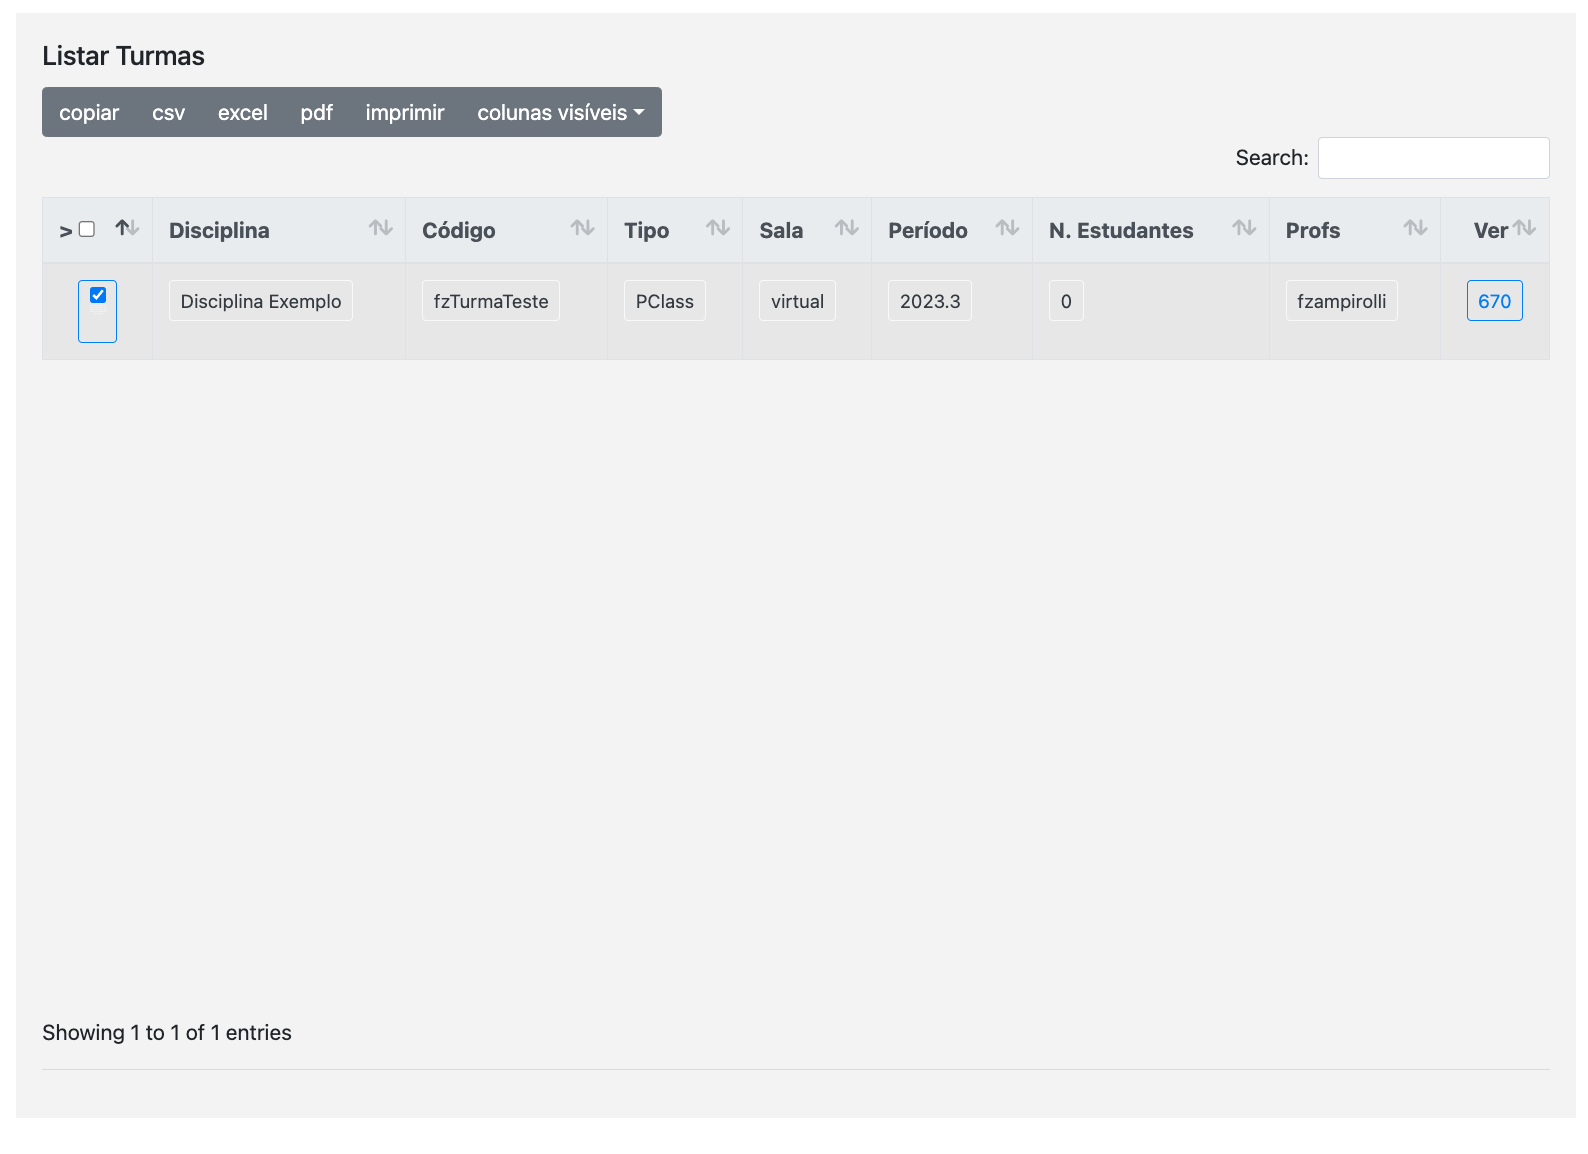
\includegraphics[width=0.9\textwidth]{cap06_figExameAtualizaTurmas.png}
  \caption{Recorte II da tela de exame, com as turmas do professor.}
  \label{fig:cap06_figExameAtualizaTurmas}\vspace{-3mm}
\end{figure}

\section{Recorte III da tela de exame -- tópicos}\label{sec:exameTopicos}

No MCTest 5.3, foi adicionada uma nova área à tela do exame, que permite a seleção dos tópicos da disciplina, ver Figura \ref{fig:cap06_figExameAtualizaTopicos}. Esse recurso se mostrou necessário, pois a tela anterior estava demorando muito para carregar todas as questões cadastradas nos tópicos da disciplina. Agora, o professor pode primeiro escolher o(s) tópico(s), clicar no botão ``Salvar'' e, no próximo Recorte IV da tela, serão apresentadas apenas as questões correspondentes ao(s) tópico(s) selecionado(s).

\begin{figure}[htbp]
  \centering
  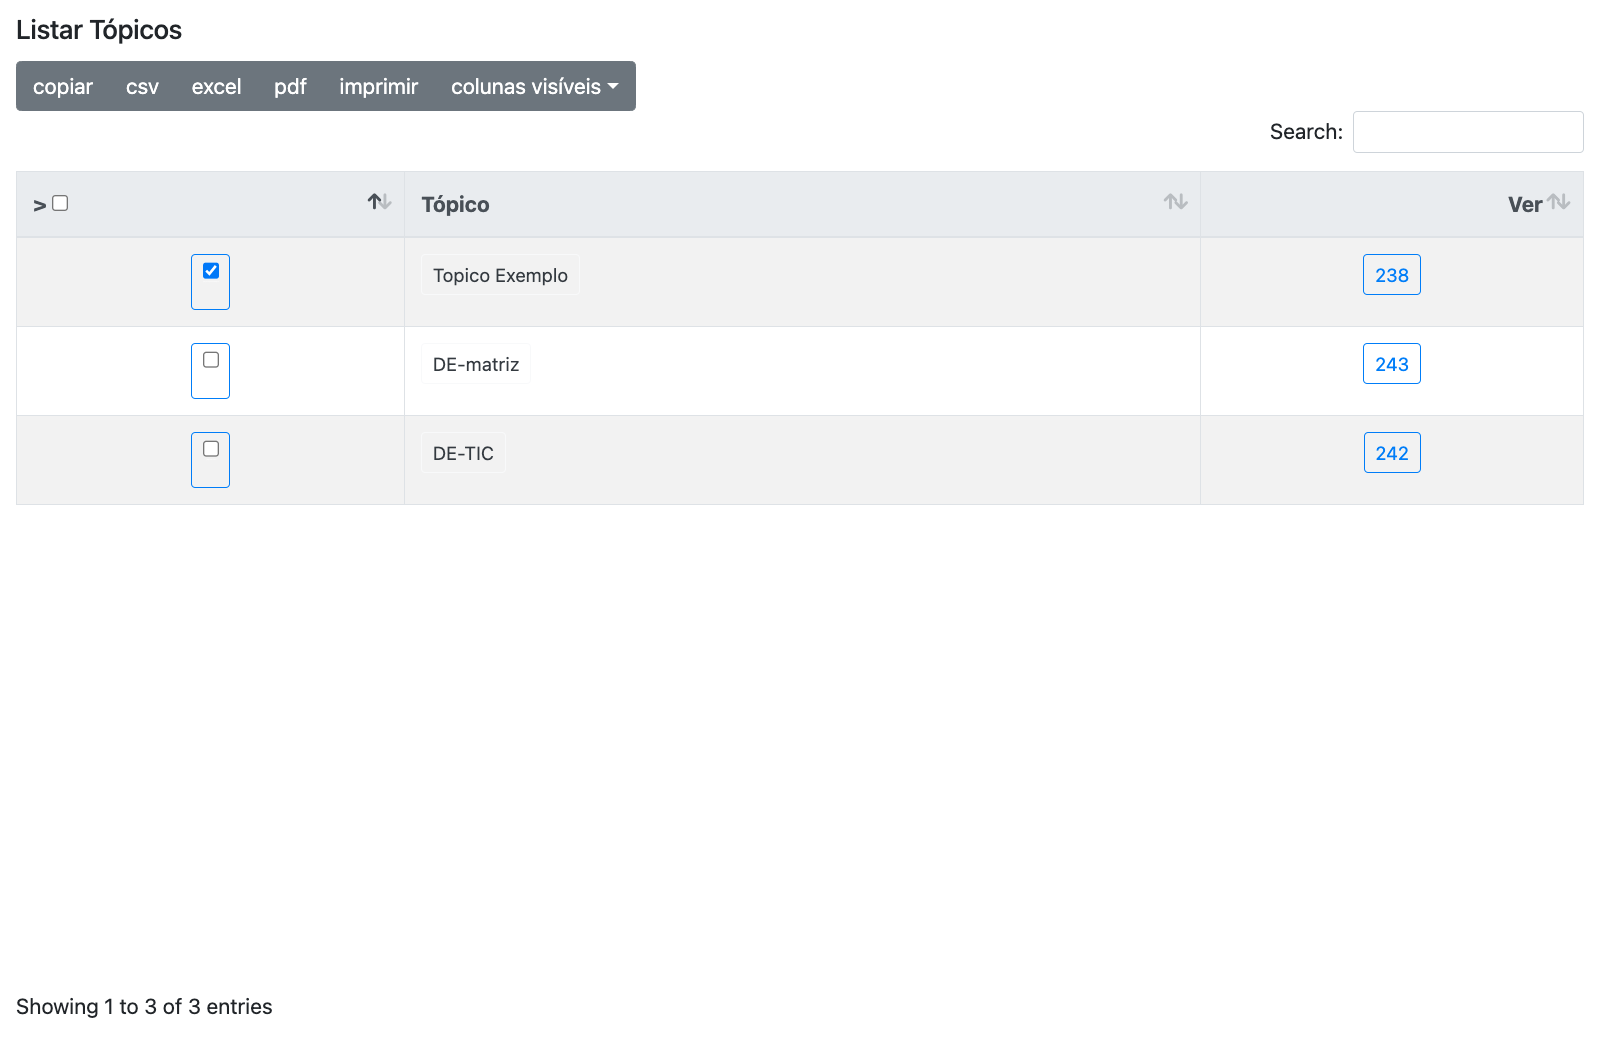
\includegraphics[width=0.9\textwidth]{cap06_figExameAtualizaTopicos.png}
  \caption{Recorte III da tela de exame, com os tópicos da disciplina.}
  \label{fig:cap06_figExameAtualizaTopicos}\vspace{-3mm}
\end{figure}

\section{Recorte IV da tela de exame -- questões}

O professor tem a opção de selecionar as questões desejadas para aplicar na avaliação, conforme ilustrado na Figura \ref{fig:cap06_figExameAtualizaQuestoes}. Essa seleção é feita marcando a caixa de seleção na primeira coluna correspondente a cada questão desejada. As questões marcadas serão sempre exibidas no topo da lista de questões, após clicar no botão "Salvar". Essa lista contém todas as questões da disciplina, dos tópicos selecionados anteriormente, à qual o exame está vinculado.

Na Figura \ref{fig:cap06_figExameAtualizaQuestoes}, também são exibidos os seguintes detalhes sobre cada questão: tópico, descrição curta, tipo QM ou QT, seguido pelo número de alternativas (é importante ressaltar que todas as questões devem ter o mesmo número de alternativas em cada exame), dificuldade (as questões de dificuldade 1 são apresentadas primeiro, seguidas pelas questões de dificuldade 2, e assim por diante; em seguida, são apresentadas as QTs, também nessa ordem), grupo (apenas uma questão por grupo é sorteada em cada exame) e, por fim, se a questão é paramétrica ou não.

A última coluna, intitulada ``Ver'', exibe o ID da questão. Ao clicar nesse botão, o professor poderá visualizar a questão em detalhes.

\begin{figure}[!t]
  \centering
  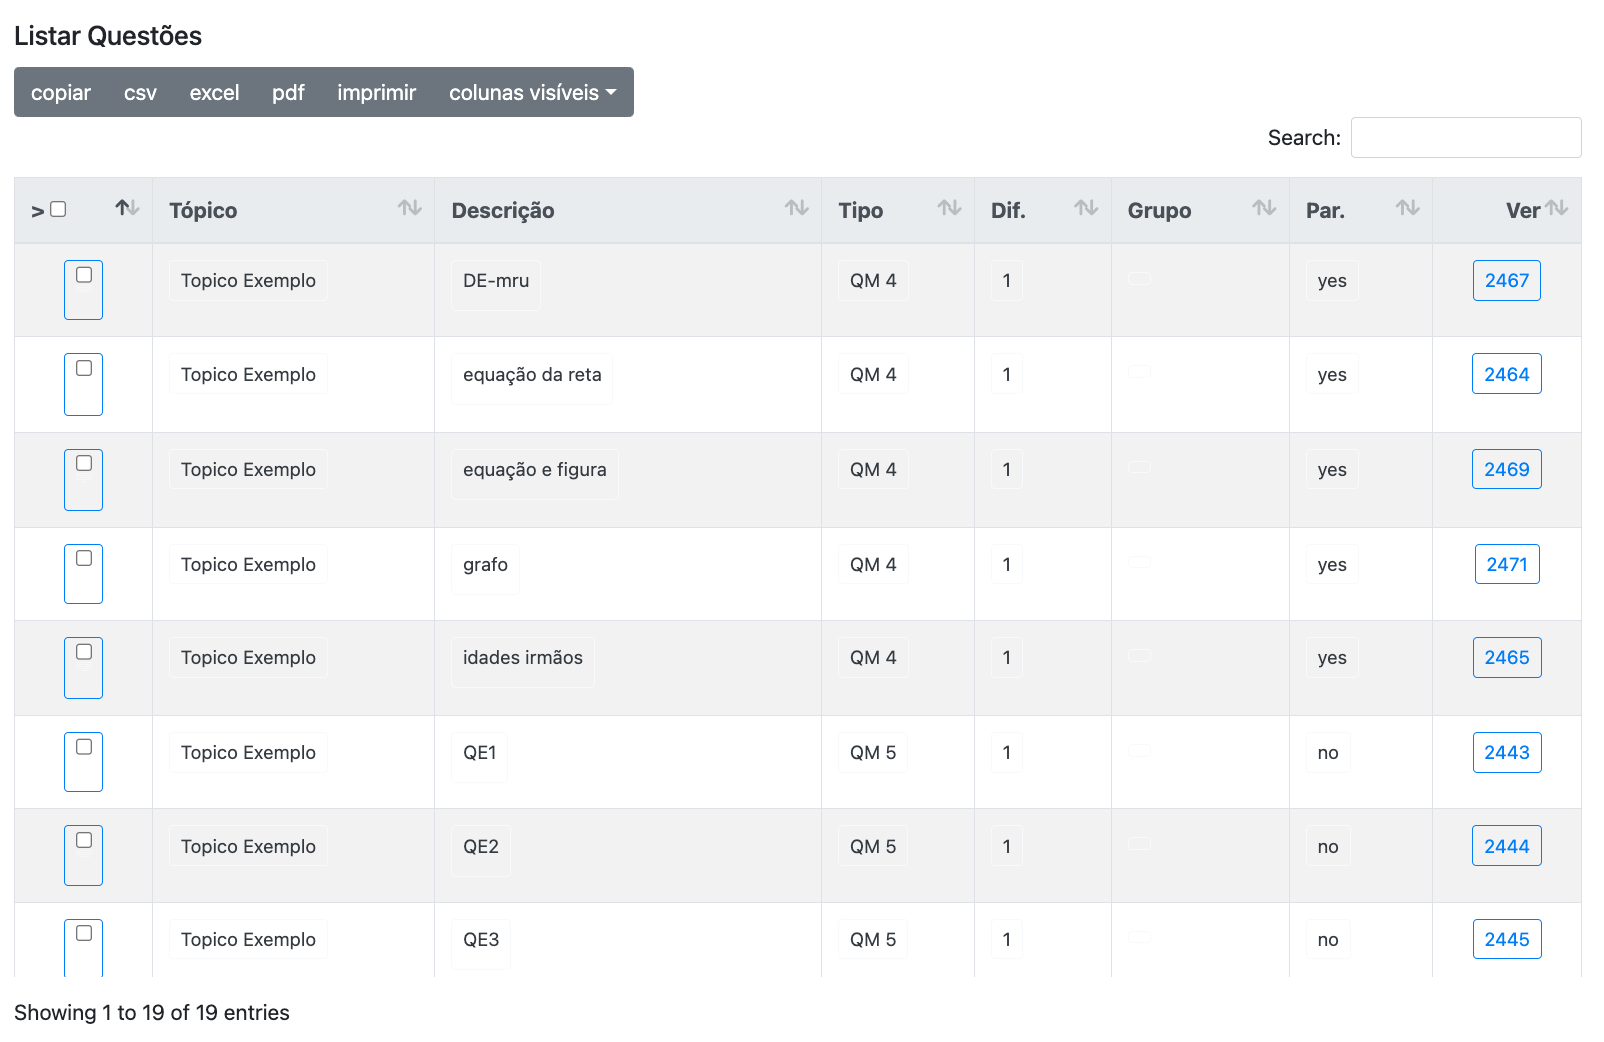
\includegraphics[width=0.9\textwidth]{cap06_figExameAtualizaQuestoes.png}
  \caption{Recorte IV da tela de exame, com as questões da disciplina, do(s) tópico(s) selecionado(s).}
  \label{fig:cap06_figExameAtualizaQuestoes}\vspace{-3mm}
\end{figure}

\section{Recorte V da tela de exame -- configurando os detalhes}\label{sec:exameDetalhes}

Na Figura \ref{fig:cap06_figExameAtualizaConfiguracoes}, são apresentados os campos de configuração de um exame. Cada questão possui uma dificuldade variando de 1 a 5. O professor deve selecionar a quantidade de QMs (na Figura \ref{fig:cap06_figExameAtualizaQuestoes}) que deseja incluir em cada exame. As questões serão exibidas em ordem crescente de dificuldade, começando pela dificuldade 1 e assim por diante. É importante observar que todas as QMs de um exame devem ter o mesmo número de alternativas. Além disso, é possível criar exames que contenham QTs, seguindo a ordem de dificuldade de cada questão.

\begin{figure}[!t]
  \centering
  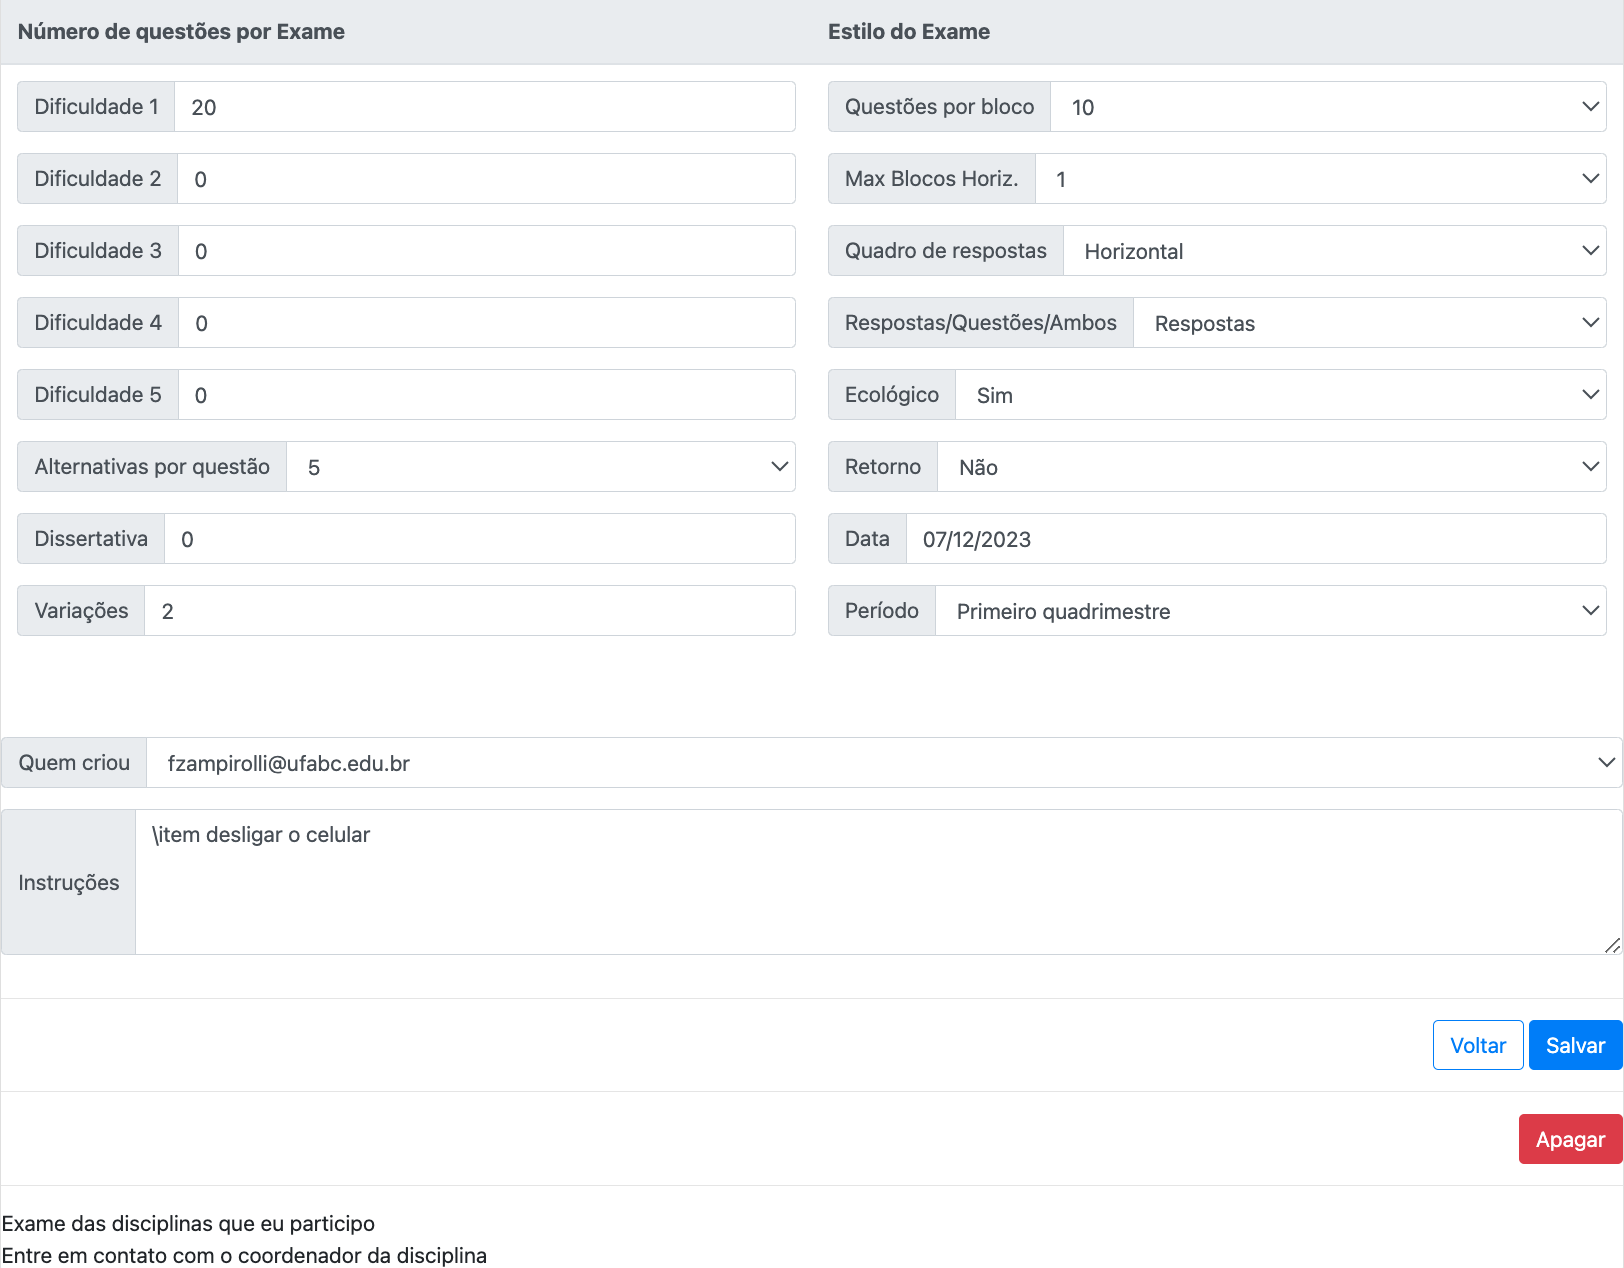
\includegraphics[width=0.9\textwidth]{cap06_figExameAtualizaConfiguracoes.png}
  \caption{Recorte V da tela de exame, configurando os detalhes do exame.}
  \label{fig:cap06_figExameAtualizaConfiguracoes}\vspace{-3mm}
\end{figure}

\begin{myboxCode}{corObs}{\textbf{Alguns exemplos de erros comuns que podem ocorrer:\\\vspace{-3mm}\hrule\vspace{3mm}}}
Na Figura \ref{fig:cap06_figExameAtualizaConfiguracoes}, o número de questões por dificuldade de 1 a 5 é aplicável apenas a QM. O número de QTs não é contabilizado por dificuldade.
Quanto ao número de questões por dificuldade:
\begin{enumerate}[itemsep=-1mm]
    \item É comum ocorrer um erro ao definir uma quantidade inferior de QMs em relação à quantidade selecionada anteriormente (Figura \ref{fig:cap06_figExameAtualizaTurmas}) para cada dificuldade, especialmente quando as questões possuem grupos. Lembre-se de que em cada exame é sorteada apenas uma questão por grupo. Portanto, se você selecionar 10 questões do grupo X, deve considerar apenas uma questão para contabilizar a quantidade correta;
    \item Também é comum ocorrer o erro de selecionar QMs com um número diferente de alternativas;
    \item Finalmente, ocorre erro ao contabilizar questões com diferentes dificuldades.
\end{enumerate}
\end{myboxCode}

Na Figura \ref{fig:cap06_figExameAtualizaConfiguracoes}, à direita, é possível visualizar o estilo do(s) bloco(s) de respostas ou QRs, onde os estudantes devem marcar as alternativas. Esses QRs aparecem na primeira folha da avaliação. Diversos estilos estão disponíveis em \href{http://vision.ufabc.edu.br/MCTest/MCTest5-Experiments/}{vision.ufabc.edu.br/MCTest/MCTest5-Experiments}. Se a opção ``Ecológico'' for definida como ``NÃO'', cada QT será desenhada em uma única folha, frente e verso.

\begin{mybox}{corCopia}{\textbf{Atenção:\\\vspace{-3mm}\hrule\vspace{1mm}}}
\begin{enumerate}[itemsep=-1mm]
    \item  Se a opção ``Retorno'' for selecionada como ``SIM'' na tela de Exame, ao pressionar o botão ``Criar-PDF'', será enviado um e-mail para cada estudante contendo o exame em um arquivo PDF anexado;
    \item Um exame só existe se estiver associado a uma turma. Portanto:
    \begin{itemize}[itemsep=-1mm]
        \item Antes de excluir as turmas, certifique-se de que todos os exames estejam associados a uma única turma. Somente após isso, você poderá excluir as outras turmas;
        \item Se um exame for deixado sem uma turma selecionada na Figura \ref{fig:cap06_figExameAtualizaTurmas} e você clicar em ``Salvar'', ocorrerá um erro. Nesse caso, será possível corrigir apenas se o administrador fizer alterações diretamente no BD, o que não é recomendado;
        \item Foram adicionadas várias mensagens de erro para tentar lidar com esses problemas.
    \end{itemize}
\end{enumerate}
\end{mybox}

\begin{myboxCode}{corObs}{\textbf{Alguns exemplos de erros comuns que podem ocorrer:\\\vspace{-3mm}\hrule\vspace{3mm}}}
Um erro frequente ocorre quando o campo ``Respostas/Questões/Ambos'' é incompatível com os demais atributos do exame. Certifique-se de que as opções selecionadas nesse campo sejam consistentes com as demais configurações do exame.
\begin{enumerate}[itemsep=-1mm]
    \item A opção ``Respostas'' exibe apenas o QRs, sem as questões. Essa opção é útil quando o professor deseja aplicar apenas QMs, mas fornece os enunciados das questões em outro documento, não gerado pelo MCTest. Nesse caso, não é possível ter variações de exame;
    \item A opção ``Questões'' é geralmente usada para avaliações com QTs;
    \item A opção ``Ambos'' permite incluir tanto o QR quanto as QMs, podendo também incluir QTs.
\end{enumerate}
\end{myboxCode}

\section{Considerações finais}

A realização dos exames desempenha um papel fundamental no MCTest, sendo o elemento central do sistema. Neste capítulo, será fornecida uma visão geral da tela de exames utilizada no MCTest, abordando os principais aspectos relacionados à criação e configuração dos exames.

Ao acessar a tela de exames, o professor tem a flexibilidade de incluir uma ou várias turmas de estudantes em um exame, selecionar as questões que farão parte dele e definir diversos aspectos relevantes, como o formato de impressão, a quantidade de variações a serem criadas e a entrega do exame aos estudantes.

Foram exploradas as diferentes seções presentes na tela de exames, destacando o processo de seleção das turmas associadas ao exame, a escolha das questões a serem incluídas e a configuração detalhada do exame, como a definição da quantidade de QMs e QTs.

Ao longo dos capítulos seguintes, serão aprofundadas as modalidades de exames disponíveis no MCTest, abordando questões com apenas o QR, questões com o enunciado completo, QTs que requerem correção manual e exames compostos por diferentes estilos de questões.

É importante estar ciente de possíveis erros comuns ao criar e configurar os exames, como a definição incorreta do número de questões por dificuldade, especialmente quando as questões possuem grupos, e a seleção de QMs com um número diferente de alternativas. O sistema conta com mensagens de erro para auxiliar na identificação e correção desses problemas.

Por fim, foi destacada a importância de associar corretamente os exames a uma turma e de verificar as configurações antes de realizar exclusões, garantindo a integridade dos dados e o correto funcionamento do sistema.

No próximo capítulo, será abordada a modalidade de exames com apenas QR, explorando suas características e funcionalidades.